\color{red}
In the last two sections we discussed linear motion in the plane and motion with a uniform vector field in the plane. Now, we understand the motion of \eqref{eq:magnetichamiltonian2}: within $S$ the motion follows an arc of a Larmor circle, and outside $S$ the motion is linear. We notice that we can describe the motion solely using analytic geometry, that is, the dynamics is determined by intersections of lines with circles or circles with circles, with the exception of trajectories that are tangent to $\partial S$ which we discussed before and have since ignored.

We present now, and prove later, that the continuous time motion of \eqref{eq:magnetichamiltonian2} can be characterized discretely, that is, we can pick a Poincar\'e section and a Poincar\'e map.
\color{black}

We notice that the dynamics of the system can be broken down into two modes: the first linear motion outside the magnetic disk, and the second being deflection in the disk. If a trajectory with initial condition on the boundary of the disk always returns to the boundary of the disk we can compress the system from continuous time to discrete time via a Poincar\'e map. We would then like to prove that the boundary of the magnetic region with the set of outward pointing velocities, that is,
\begin{align}\label{def:poincaresection}
S = \bigcup_{\theta\in[0,2\pi]}\{\theta\}\times\left[\theta-\frac{\pi}{2},\theta+\frac{\pi}{2} \right]
\end{align}
is a Poincar\'e section. To prove this we need to recall rotations on a torus. If the angle of rotation is irrational, then the trajectory fills the torus densely, if the angle is rational, then the trajectory is periodic and a closed loop. To complete the statement, we need the Poincar\'e map $P$ itself, \color{red}here we state the form of the map but we are too lazy for now.\color{black}

We define the map $P$ already assuming that the trajectory returns for sure. We prove that it does now:

\begin{proposition}
The set $S$ as in \eqref{def:poincaresection} is a Poincar\'e section for the system, and the map $P:U\to P(U)$ is a Poincar\'e map.
\end{proposition}

\begin{proof}
We need to prove that a trajectory of the system with initial condition in $S$ returns to $S$. Notice that if a trajectory enters the disk transversally, it will exit the disk transversally as well. This means if we can show that if all initial conditions in $S$ have a time $t$ at which their trajectory is on the disk and is pointing inward, then we are done.

Let $(x,v)\in S$, and consider the trajectory of the system evolving with this initial condition. If $v$ is a rational angle, then the trajectory corresponding to rotations on the torus is periodic, and there exists a time $t>0$ at which we return to the same point $x$. Since $(x,v)$ is transversal to the disk, this means there exists a time $t_1<t$ when the trajectory is on the boundary of the disk and has velocity pointing inward the disk.

If $v$ is an irrational angle, then the trajectory corresponding to rotations on the torus is dense in the torus. Let $U$ be a neighborhood of $x$ in the boundary of the disk, such that all $U\times\{v\}$ are transversal to the disk. This is possible, since $(x,v)$ itself is transversal. Pick $y\in U$, then for some $t>0$ the trajectory of the rotation is at $y$ with velocity $v$, that is the trajectory is transversal. Following the same reasoning as the previous case, there is a time $t_1<t$ at which the trajectory must enter the disk.

We have shown that the trajectory of the rotation returns to the disk and points inward in finite time, and at least once. For the Poincar\'e map we then take the first time the trajectory returns to the disk. 
\end{proof}

Using the Poincar\'e map we can study the stability of periodic trajectories of the system. The computations become unwieldy on paper, so we use a computer. The code for this can be found at \color{red}insert code reference [??]\color{black}

The code written in \texttt{Python} utilizes the symbolic algebra system \texttt{Sympy} to define functions, compute derivatives, compose functions, and compute eigenvalues of a Jacobian symbolically. That way we avoid a considerable amount of computation by hand but still retain a high degree of precision when computing numerical values. For long enough periodic orbits, the computation time using symbolic algebra becomes unreasonable, so we require a different way to analyse stability. A common alternative is to compute Lyapunov exponents of the original system or of the Poincar\'e map. However, these approaches are prone to numerical instability and require significant preparation beforehand. We would like to analyze stability from the trajectory directly, and we attempt this via symbolic dynamics in the next section.


\color{red}
With $B_r(q)\subset \mathbb R^2$ denote the closed ball of radius $r>0$ centered at $q\in\mathbb R^2$. Pick $S=\cup_{N\in\mathbb Z^2}B_{1/3}(N-1/2)$, that is, $S$ is the union of closed balls of radius $1/3$ centered at points of the form $(n-1/2,m-1/2)$ for $n,m\in\mathbb Z$.

The choice of radius $r=1/3$ is arbitrary, we fix it for convenience. Furthermore, we notice the speed of the particle is constant, since $\|X'(0)\|=Rb$, so again for simplicity we fix $\|X'(0)\|=1$. This also fixes the Larmor radius $R=1/b$. A different choice of $r\in (0,1/2)$ and $\|X'(0)\|\in(0,\infty)$ clearly gives rise to different dynamics, however we make the assumption that the dynamics will not differ \textit{qualitatively}, i.e., in any case we expect to find periodic orbits, chaotic behavior, and the methods we use for studying these are still valid.

Hence, we study the influence of varying the parameter $b>0$ on the above defined system. What we see is four ranges of behavior:
\begin{enumerate}
\item For values $b\approx0$ we can approximate the dynamics as a perturbation of a system with no magnetic field at all,
\item For a range of ``small'' values of $b$, the dynamics are similar to that of a uniform field in $\mathbb R^2$,
\item there is an intermediate range where both stable and unstable periodic dynamics occur
\item there exists a value $b_t$, such that all values $b>b_t$ give rise to unstable dynamics.
\end{enumerate}

We can use this to already find some simple periodic orbits. We describe one such orbit now.

Let $\delta\in(0,1/3)$ and consider the initial condition $(x,p) = (0,1/2+delta,1,0)$, the trajectory can be seen in \cref{subfig:periodicorbit1}. We can compute that for the choice $b=1/\delta$, the trajectory will be a periodic orbit.

Already, we see that periodic orbits exist for arbitrarily large $b$. It can be shown using Poincar\'e sections that this family of periodic orbits is unstable.

Another family of periodic orbits are given for $\delta\in(-1/\sqrt{18},1/3)$, where the initial condition is $(x,p)=(0,1/2+\delta,1,0)$ and $b = 1/(\delta+\sqrt{1/9-\delta^2})$

Another family of periodic orbits are given for $\delta\in(1/\sqrt{18},1/3)$, where the initial condition is $(x,p)=(0,1/2+\delta,1,0)$ and $b = 1/(\delta-\sqrt{1/9-\delta^2})$

Lastly, we have a more complicated periodic orbit that forms an octagon for 


\begin{figure}[!th]
\centering
\begin{subfigure}{0.49\textwidth}
\centering
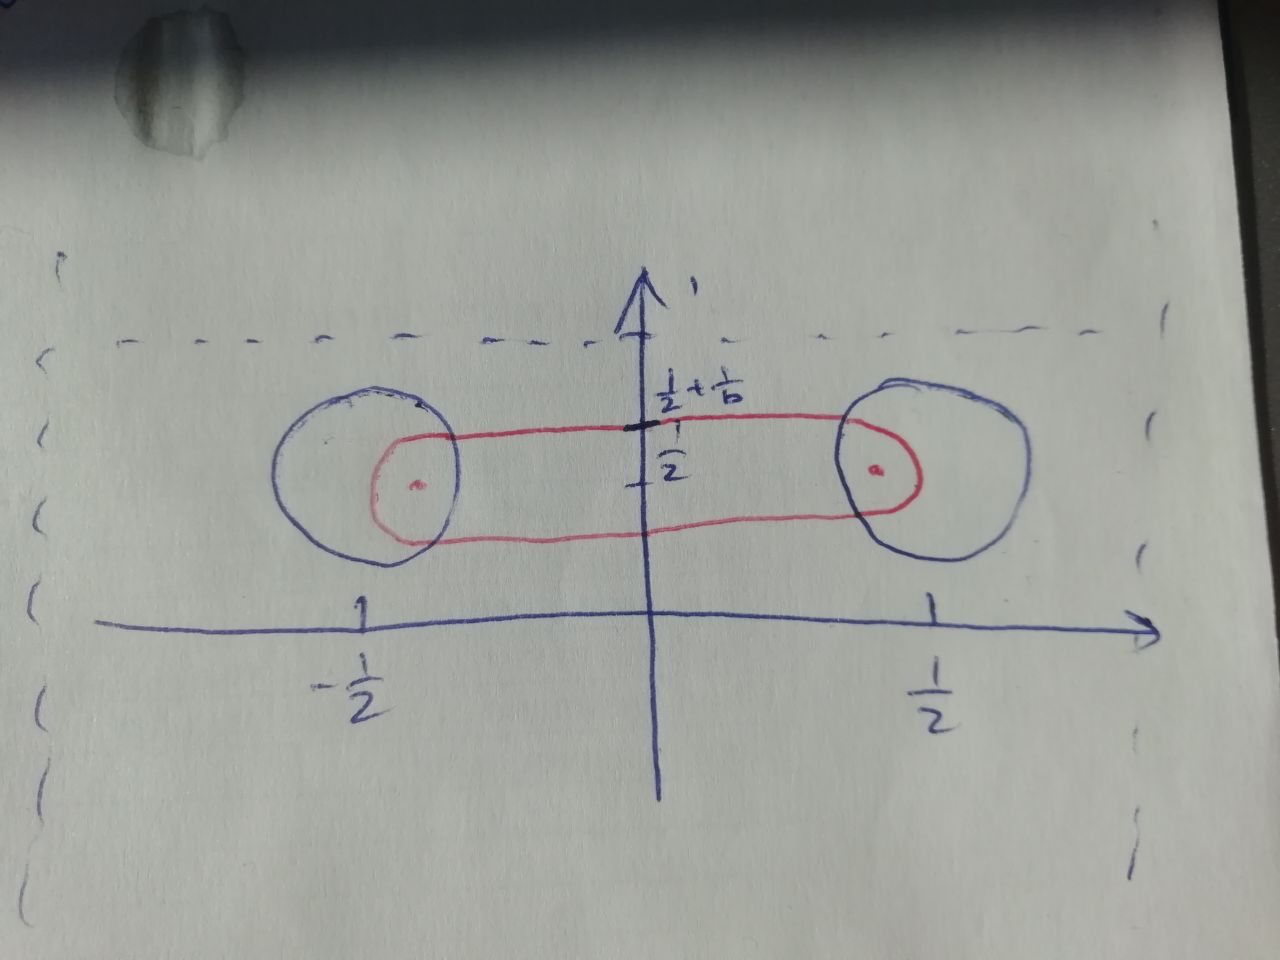
\includegraphics[width=\textwidth]{photo_2023-04-17_18-09-20.jpg}
\caption{$(x,p) = (0,1/2+\delta,1,0)$ and $b=1/\delta$ where $\delta\in(0,1/3)$.}
\label{subfig:periodicorbit1}
\end{subfigure}
%
\begin{subfigure}{0.49\textwidth}
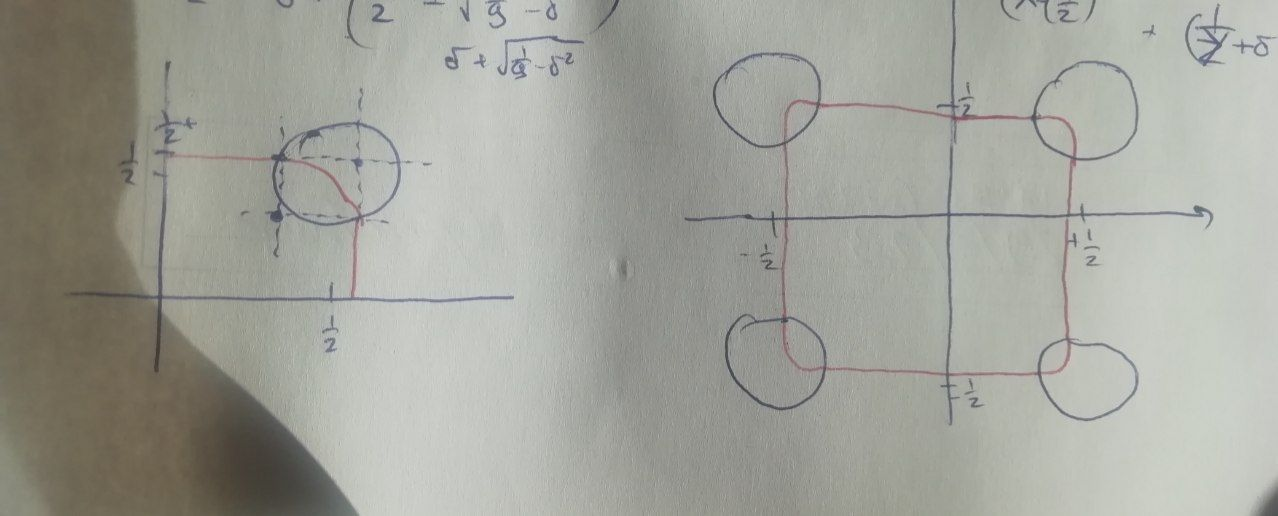
\includegraphics[width=\textwidth, trim={20cm 0 0 0}, clip]{photo_2023-04-17_18-09-21.jpg}
\caption{$(x,p) = (0,1/2+\delta,1,0)$ and $b=1/(\delta+\sqrt{1/9-\delta^2})$ where $\delta\in(-1/\sqrt{18},1/3)$.}
\label{subfig:periodicorbit2}
\end{subfigure}
%
\begin{subfigure}{0.49\textwidth}
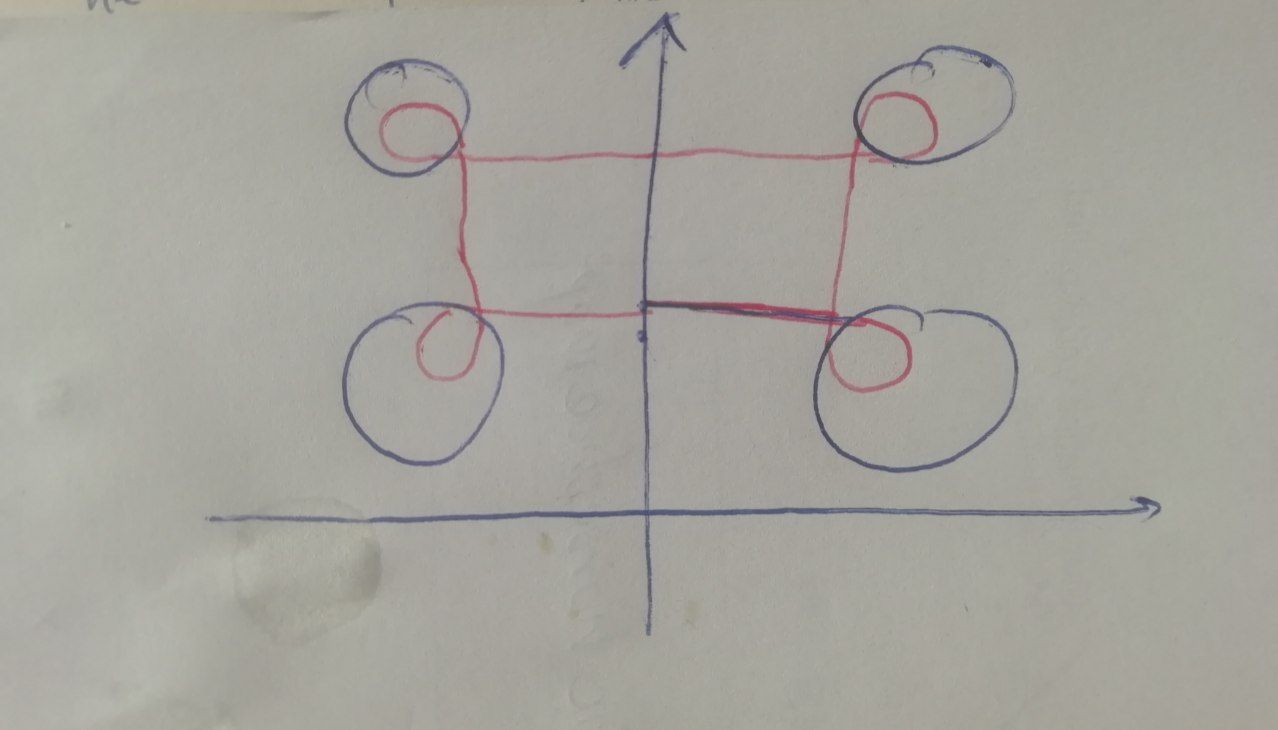
\includegraphics[width=\textwidth]{photo_2023-04-17_18-09-23.jpg}
\caption{$(x,p) = (0,1/2+\delta,1,0)$ and $b=1/(\delta-\sqrt{1/9-\delta^2})$ where $\delta\in(1/\sqrt{18}),1/3$.}
\label{subfig:periodicorbit3}
\end{subfigure}
%
\begin{subfigure}{0.49\textwidth}
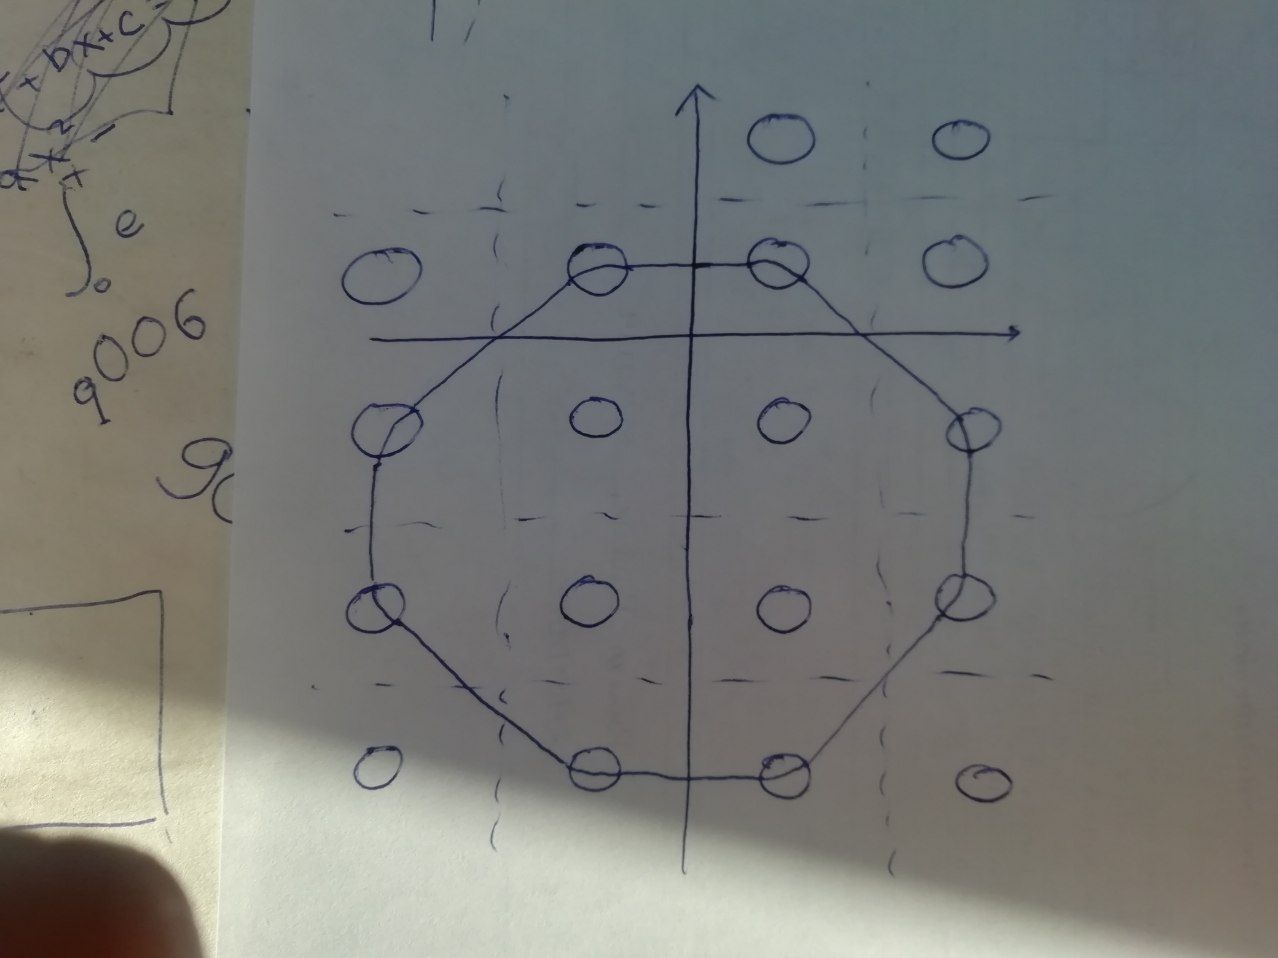
\includegraphics[width=\textwidth]{photo_2023-04-17_18-41-12.jpg}
\caption{$(x,p) = (0,1/2+\delta,1,0)$ and $b=1/(\delta-\sqrt{1/9-\delta^2})$ where $\delta\in(1/\sqrt{18}),1/3$.}
\label{subfig:periodicorbit4}
\end{subfigure}
\caption{Some families of periodic orbits with initial condition $(x,p)$ and magnetic field strength $b$, parametrized by $\delta>0$.}
\label{fig:periodicorbits}
\end{figure}

\color{black}